
\subsection{Snubber-kredsløb}
Der blev designet to snubber-kredsløb for, at fjerne ringninger på spændingen over både MOSFET og diode. De blev anslået som en konsekvens af at spredningsselvinduktionen fremstår som en serie forbindelse med kapaciteten over henholdsvis MOSFET'en, dioden og den kapacitive kobling mellem transformatorens viklinger.  

Det blev valgt at implementere RC-snubbere til både primær- og sekundærsiden. De består af en modstand i serie med en kondensator, som skal placeres over henholdsvis MOSFET og diode. 

Med kendskab til ringningernes frekvens på primærsiden og transformatorens spredningsselvinduktion, blev den resulterende kapacitet regnet til $266.6pF$. Kondensatoren i snubber-kredsløbet blev valgt til en faktor 2 større end den resulterende kapacitet, for optimal funktionalitet\cite{snubber_design}. Modstanden blev designet således impedansen var lig impedansen af spredningsselvinduktionen ved ringningsfrekvensen. Hermed blev snubber-kredsløbet designet til $C_{snubM} = 600pF$ og $R_{snubM} = 23.7\ohm$. 

Figur~\ref{fig:snubber_diagram} viser implementeringen af de to snubber kredsløb. Her vises de specifikke komponentværdier og placeringen af de to snubber-kredsløb.

\begin{figure}[H]
	\centering
	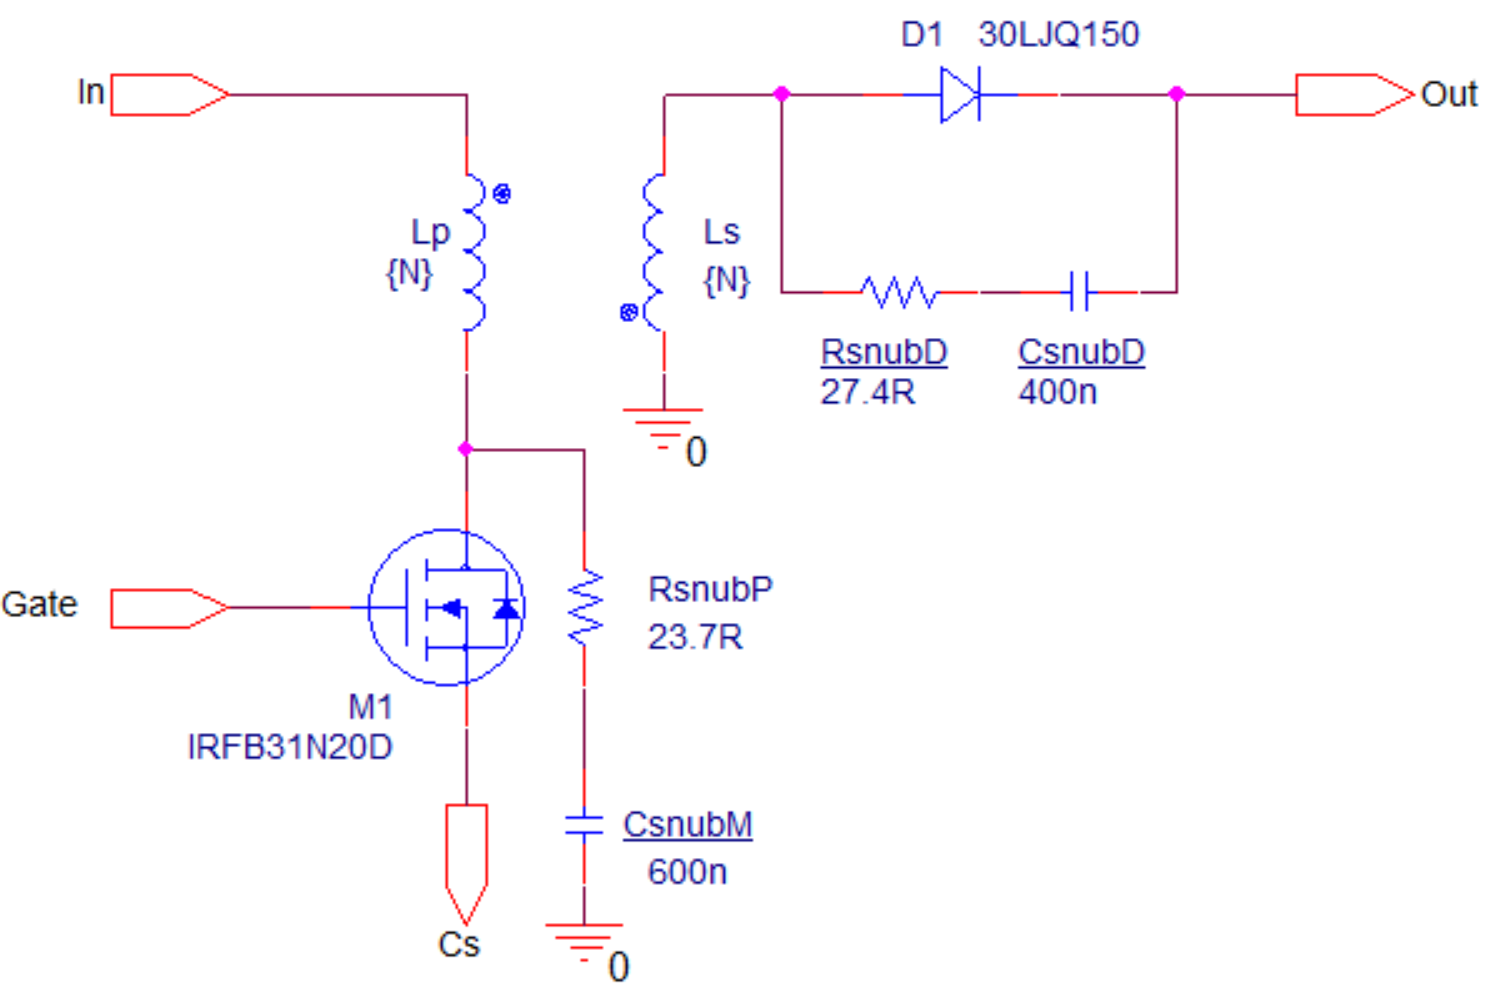
\includegraphics[width=0.7\linewidth]{/tex/Implementering/3iteration/Billeder/Snubber_diagram.png}
	\caption{P-spice diagram for snubber-kredsløb}
	\label{fig:snubber_diagram}
\end{figure}

Designmetoden for snubber-kredsløbet på sekundærsiden er den samme. Der findes en detaljeret gennemgang af designproceduren og en argumentation for valg snubber type i dokumentationens afsnit 6.3.
